\section{Results}
\label{sec:results}

We ask four questions about the meaning preserved by the tokenizer.
What does a tokenized concept look like (Section~\ref{sec:results:examples})?
Does our selection preserve meaning better than graph-based selections, and how do $k$ and $\lambda$ matter (Section~\ref{sec:results:benchmark})?
On real, long-tailed EHR data, are rare concepts preserved (Section~\ref{sec:results:hero})?
Do semanticians agree with the automatic metrics (Section~\ref{sec:results:expert})?

% ------------------------------------------------------------------
\subsection{Experimental setup}
\label{sec:setup}

We run two experiments with the same pipeline on two concept sets, each with its own candidate subgraph and candidate pool (Table~\ref{tab:setup}).
The benchmark uses no patient data; the EHR application uses real event counts.

\paragraph{Benchmark on the mapped concepts.}
The benchmark uses the set $M$ of 46,150 SNOMED~CT concepts to which the codes of the clinical data warehouse of the Geneva University Hospitals (HUG) were mapped by the institution's terminology experts \notetoself{SNOMED CT release used}.
It relies only on these concepts and on the ontology graph.
We set the hop radius to $D = 9$, which covers 98.4\% of the concept depths in the candidate subgraph.
The resulting subgraph $G_D$ is a DAG that keeps 103 of the 113 relationship types (Appendix~\ref{app:relations}).
Its 75,964 nodes form the candidate pool: the 46,150 mapped concepts and the 29,814 concepts they reach.
All 19 configurations of Section~\ref{sec:method:baselines} select their tokens from this pool, at the budgets $k = 500, 1{,}000, \dots, 19{,}500$, which we group into three compression levels of 13 budgets each (Table~\ref{tab:setup}b).

\paragraph{Application to real EHR data.}
The second experiment uses the structured patient data of the HERO project at HUG, collected between 2017 and 2025 \notetoself{ethics approval / general consent}.
Of the 18,687 distinct SNOMED~CT codes in the data, 16,370 are concepts of our graph and form the set $\Mhero$; the other 2,317 are missing from the relationship table we use.
The concepts of $\Mhero$ occur in 279 million events from 937,096 patients.
We ran the whole pipeline again on $\Mhero$ alone, with the same hop radius $D = 9$, which gives a smaller candidate pool than in the benchmark (Table~\ref{tab:setup}a).
Token budgets are therefore not comparable between the two experiments: $k = 5{,}000$ is 10.8\% of $|M|$ but 30.5\% of $|\Mhero|$.
We evaluate budgets from $k = 250$ to $k = |\Mhero| = 16{,}370$ and compare our tokenizer with frequency truncation (Section~\ref{sec:method:ehr}).

\paragraph{Expert evaluation.}
Semanticians compared our tokenizer with Personalized PageRank at $k = 5{,}000$ on a stratified sample of 100 concepts of $\Mhero$, blinded, with the official SNOMED~CT definition as reference (Section~\ref{sec:method:expert}).

\begin{table}[t]
\centering
\small
\caption{Experimental setup. (a) Full SNOMED~CT graph $G$ and the two experiments, each with its own candidate subgraph ($D = 9$). (b) Compression levels of the benchmark; each level contains 13 token budgets in steps of 500.}
\label{tab:setup}
\begin{tabular}{@{}lrrr@{}}
\toprule
\multicolumn{4}{@{}l}{\textit{(a) Graphs and experiments}} \\
 & Full graph $G$ & Benchmark ($M$) & HERO ($\Mhero$) \\
\midrule
Concepts to represent & --        & 46,150      & 16,370 \\
Candidate pool (nodes)& 447,420   & 75,964      & 37,601 \\
Edges                 & 1,684,197 & 293,146     & 134,313 \\
Relationship types    & 113       & 103         & 87 \\
Token budgets $k$     & --        & 500--19,500 & 250--16,370 \\
Compared with         & --        & 18 other configurations & frequency truncation \\
\midrule
\multicolumn{4}{@{}l}{\textit{(b) Compression levels of the benchmark}} \\
Level & $k$ & $k/|M|$ (\%) & \\
\midrule
High & 500--6,500     & 1.1--14.1  & \\
Mid  & 7,000--13,000  & 15.2--28.2 & \\
Low  & 13,500--19,500 & 29.3--42.3 & \\
\bottomrule
\end{tabular}
\end{table}

% ------------------------------------------------------------------
\subsection{What a tokenized concept looks like}
\label{sec:results:examples}

Before comparing selection methods, we show what our tokenizer produces for three mapped concepts and how the metrics read on each of them (Figure~\ref{fig:example-trees}, Table~\ref{tab:example-trees}).
We fix $\lambda = 0.9$ and $k = 5{,}000$ ($k/|M| = 10.8\%$) for illustration only; Section~\ref{sec:results:benchmark} studies both parameters.
We chose concepts with shallow trees for readability.

\textit{Pain of breast} (Figure~\ref{fig:example-trees}a) has three outgoing relationships: a \textit{finding site} edge to \textit{breast structure}, and two \isa{} edges, to \textit{chest pain} and to \textit{finding of sensation of breast}.
Breast structure and chest pain are tokens at depth~1.
Finding of sensation of breast is not a token, so \textsc{Expand} continues through its two parents, \textit{finding of sensation by site} and \textit{breast finding}, which are tokens at depth~2.
Because \isa{} is transparent, these three tokens join the initial context, whereas the finding site opens a subcontext that holds breast structure.
Finding of sensation of breast has the same finding site as its child; since this pair is already in the initial context, it is not expanded again (dashed edge).
The resulting tree is
\[
\big(\textit{finding of sensation by site},\ \textit{breast finding},\ \textit{chest pain},\ \textit{finding site}(\textit{breast structure})\big).
\]
All four branches end at a token ($c_m = 1$) at a mean depth of 1.5, so the concept keeps most of its meaning, with $\mathrm{PC}_m = 1 - 1.5/10 = 0.85$, and no other concept shares its tree.

\textit{Hyperthyroidism} and \textit{sick-euthyroid syndrome} (Figure~\ref{fig:example-trees}b) have the same two relationships: an \isa{} edge to \textit{disorder of thyroid gland} and a \textit{finding site} edge to \textit{thyroid structure}.
Both targets are tokens at depth~1, so both concepts receive the same tree,
\[
\big(\textit{disorder of thyroid gland},\ \textit{finding site}(\textit{thyroid structure})\big).
\]
Each tree scores well on its own ($\mathrm{PC}_m = 0.90$), yet a downstream model cannot tell the two concepts apart, although they describe different conditions: an overactive thyroid gland, and abnormal thyroid tests with a normal gland.
Both concepts are primitive: the graph does not state what distinguishes them, so no token set can separate them unless one of them becomes a token itself (Section~\ref{sec:limitations}).

\begin{figure}[t]
\centering
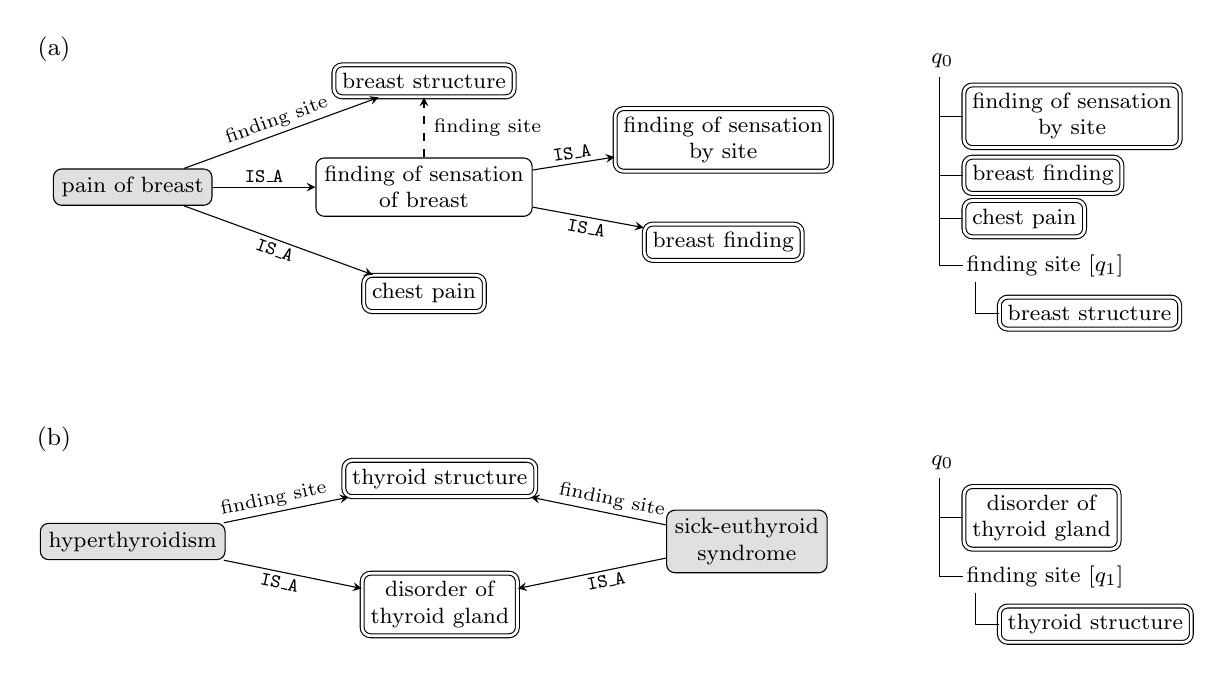
\begin{tikzpicture}[
  >=stealth,
  concept/.style={draw, rounded corners=3pt, align=center, font=\footnotesize, inner sep=3pt},
  mapped/.style={concept, fill=black!12},
  token/.style={concept, double, double distance=1pt},
  rel/.style={font=\scriptsize, sloped, above, inner sep=1.5pt},
  isa/.style={font=\scriptsize\ttfamily, sloped, above, inner sep=1.5pt},
  treeline/.style={draw, thin},
  ctx/.style={font=\footnotesize, anchor=west, inner sep=1pt},
]
% ---------------- (a) Pain of breast ----------------
\node[font=\small] at (-1.0, 1.75) {(a)};
\node[mapped] (pb) at (0,0) {pain of breast};
\node[token]   (bs)  at (3.7, 1.35) {breast structure};
\node[concept] (fsb) at (3.7, 0)    {finding of sensation\\ of breast};
\node[token]   (cp)  at (3.7,-1.35) {chest pain};
\node[token]   (fss) at (7.5, 0.6)  {finding of sensation\\ by site};
\node[token]   (bf)  at (7.5,-0.7)  {breast finding};
\draw[->] (pb) -- node[rel] {finding site} (bs);
\draw[->] (pb) -- node[isa] {IS\_A} (fsb);
\draw[->] (pb) -- node[isa,below] {IS\_A} (cp);
\draw[->] (fsb) -- node[isa] {IS\_A} (fss);
\draw[->] (fsb) -- node[isa,below] {IS\_A} (bf);
\draw[->,dashed] (fsb) -- node[font=\scriptsize, right] {finding site} (bs);
% context tree (a)
\begin{scope}[shift={(10.1,1.6)}]
  \node[ctx] at (0,0) {$q_0$};
  \node[token,anchor=west] (a1) at (0.45,-0.7)  {finding of sensation\\ by site};
  \node[token,anchor=west] (a2) at (0.45,-1.45) {breast finding};
  \node[token,anchor=west] (a3) at (0.45,-2.0)  {chest pain};
  \node[ctx]               (a4) at (0.45,-2.6)  {finding site [$q_1$]};
  \node[token,anchor=west] (a5) at (0.9,-3.2)   {breast structure};
  \foreach \n in {a1,a2,a3,a4} \draw[treeline] (0.15,-0.2) |- (\n.west);
  \draw[treeline] (0.6,-2.8) |- (a5.west);
\end{scope}
% ---------------- (b) Hyperthyroidism and sick-euthyroid syndrome ----------------
\begin{scope}[shift={(0,-4.5)}]
\node[font=\small] at (-1.0, 1.3) {(b)};
\node[mapped] (hy) at (0,0)    {hyperthyroidism};
\node[token]  (ts) at (3.9, 0.8) {thyroid structure};
\node[token]  (dt) at (3.9,-0.8) {disorder of\\ thyroid gland};
\node[mapped] (se) at (7.8,0)  {sick-euthyroid\\ syndrome};
\draw[->] (hy) -- node[rel, pos=0.42] {finding site} (ts);
\draw[->] (hy) -- node[isa, below, pos=0.42] {IS\_A} (dt);
\draw[->] (se) -- node[rel, pos=0.42] {finding site} (ts);
\draw[->] (se) -- node[isa, below, pos=0.42] {IS\_A} (dt);
% shared context tree (b)
\begin{scope}[shift={(10.1,1.0)}]
  \node[ctx] at (0,0) {$q_0$};
  \node[token,anchor=west] (b1) at (0.45,-0.7)  {disorder of\\ thyroid gland};
  \node[ctx]               (b2) at (0.45,-1.45) {finding site [$q_1$]};
  \node[token,anchor=west] (b3) at (0.9,-2.05)  {thyroid structure};
  \foreach \n in {b1,b2} \draw[treeline] (0.15,-0.2) |- (\n.west);
  \draw[treeline] (0.6,-1.65) |- (b3.west);
\end{scope}
\end{scope}
\end{tikzpicture}
\caption{Context trees of three mapped concepts at $\lambda = 0.9$ and $k = 5{,}000$. Left: the part of $G_D$ explored by \textsc{Expand}; mapped concepts are shaded and double-bordered concepts are tokens. Right: the resulting context tree. (a) \textit{Pain of breast} receives a unique tree; the dashed edge is a finding site that its parent restates, which is not expanded again. (b) \textit{Hyperthyroidism} and \textit{sick-euthyroid syndrome} reach the same two tokens through the same relationships, and therefore share one context tree.}
\label{fig:example-trees}
\end{figure}

\begin{table}[t]
\centering
\small
\caption{Per-concept values for the examples of Figure~\ref{fig:example-trees} ($\lambda = 0.9$, $k = 5{,}000$, $D = 9$). $n_m$: tokens; $u_m$: uncovered branches; PC: proximity-coverage score; $N_{\sigma_m}$: number of mapped concepts with the same tree.}
\label{tab:example-trees}
\begin{tabular}{@{}lllcclcc@{}}
\toprule
Concept & SCTID & Status & $n_m$ & $u_m$ & Token depths & PC & $N_{\sigma_m}$ \\
\midrule
Pain of breast          & 53430007  & fully defined & 4 & 0 & 1, 1, 2, 2 & 0.85 & 1 \\
Hyperthyroidism         & 34486009  & primitive     & 2 & 0 & 1, 1       & 0.90 & 2 \\
Sick-euthyroid syndrome & 237542005 & primitive     & 2 & 0 & 1, 1       & 0.90 & 2 \\
\bottomrule
\end{tabular}
\end{table}

% ------------------------------------------------------------------
\subsection{Comparison with graph-based selection, and effect of \texorpdfstring{$k$ and $\lambda$}{k and lambda}}
\label{sec:results:benchmark}

The examples show single concepts; we now evaluate the 19 configurations on all 46,150 mapped concepts.

\paragraph{Ranking.}
At each token budget, we rank the 19 configurations on each of the four core metrics, average the four ranks, and then average over the 13 budgets of each compression level (Appendix~\ref{app:ranking}).
No configuration wins every metric.
Our method with $\lambda = 0.9$ obtains the best average rank at every compression level, and every $\lambda$ from 0.6 to 0.9 outranks all baselines (Figure~\ref{fig:rank-by-family}).
The best baselines are highest degree ($d \le 1$) among the degree-based methods and Personalized PageRank among the centrality-based ones.
The set-cover ablation ranks below every $\lambda > 0$ at every level, close to random selection.
Since it uses the same greedy procedure with a binary objective, the distance-aware objective, not greedy selection alone, drives the result.
The two extremes, $\lambda = 0$ and $\lambda = 1$, also rank near the bottom (Section~\ref{sec:discussion:why}).

\begin{figure*}[t]
\centering
\includegraphics[width=\textwidth]{paper/imgs/rank_by_family.png}
\caption{Average rank of the 19 configurations at each compression level (rank 1 = best), averaged over the four core metrics and the 13 token budgets per level. Gray points are baselines, with methods of the same family sharing a column; coloured points are our method at each value of the distance decay $\lambda$. The circled point marks the best configuration at each level ($\lambda = 0.9$ throughout).}
\label{fig:rank-by-family}
\end{figure*}

\paragraph{Effect of the token budget $k$.}
All methods follow the same trends (Figure~\ref{fig:metrics-vs-k}): the PC score and the unique rate increase with $k$, the number of tokens per concept decreases, and the unknown rate reaches zero early.
A larger vocabulary brings the nearest token closer to each concept, so branches stop earlier, which shortens the trees, and closer tokens are more specific, which separates more concepts.
Our method keeps the highest PC score at every budget and leaves no concept without a token, whereas highest degree ($d \le 1$) leaves unknown concepts up to mid compression.
The set-cover ablation has the lowest PC score and unique rate, and the longest trees, at every $k$.
The per-concept distributions show where the gain of a larger budget goes (Figure~\ref{fig:dist-k-lambda}).
For a typical concept, little changes: the median PC score rises only slightly, and the median number of tokens stays at four to five.
The gain goes to the worst-represented concepts: from high to low compression, the 10th percentile of the PC score rises from 0.62 to 0.83, and the 90th percentile of the number of tokens falls from 22 to 8.

\begin{figure*}[t]
\centering
\includegraphics[width=\textwidth]{paper/imgs/metrics_vs_k.png}
\caption{Core metrics as a function of the token budget $k$ for our method ($\lambda = 0.9$), the set-cover ablation, and the best baseline of each family (Personalized PageRank; highest degree, $d \le 1$).
Arrows indicate the preferred direction; vertical lines separate the high, mid and low compression levels (Table~\ref{tab:setup}b).
Random selection is in Appendix Figure~\ref{fig:metrics-vs-k-all}.}
\label{fig:metrics-vs-k}
\end{figure*}

\paragraph{Effect of the distance decay $\lambda$.}
Figure~\ref{fig:dist-k-lambda} compares three values of $\lambda$ between 0 and 1 with $\lambda = 1$, at one budget per compression level; Appendix~\ref{app:lambda} gives the mean metrics for every $\lambda$, including $\lambda = 0$.
From $\lambda = 0.3$ to $0.9$, the median PC score barely changes, but its lower tail rises: fewer concepts are left with only distant tokens.
The number of tokens changes little.
At $\lambda = 1$, the whole distribution of the PC score shifts down, not only its lower tail, the trees become longer, and the unique rate drops sharply (Table~\ref{tab:lambda}), at every budget.
The decay should therefore lie strictly between 0 and 1, and within this range a larger $\lambda$ mainly helps the worst-represented concepts; Section~\ref{sec:discussion:why} explains why both extremes fail.

\begin{figure*}[t]
\centering
\includegraphics[width=\textwidth]{paper/imgs/dist_k_lambda.png}
\caption{Per-concept scores of our method on the mapped concepts $M$, at one token budget per compression level ($k/|M| = 7.6\%$, $21.7\%$ and $35.8\%$) and four values of the decay $\lambda$.
(a)~Proximity-coverage score and (b)~tokens per concept: boxes span the 25th to 75th percentiles, thick lines mark the median, whiskers the 10th and 90th percentiles, and dots the mean.
The PC score takes discrete values; many concepts score exactly 0.9 (all tokens one hop away) or 1 (the concept is itself a token).
No concept is unknown in these settings, except 0.06\% at $k = 3{,}500$, $\lambda = 0.3$.}
\label{fig:dist-k-lambda}
\end{figure*}

In short, distance-aware greedy selection preserves the meaning of the mapped concepts better than every degree-, centrality- and set-cover-based selection, and a larger budget or a decay closer to (but below) 1 mainly helps the concepts that are worst represented.

% ------------------------------------------------------------------
\subsection{Rare concepts in real EHR data}
\label{sec:results:hero}

The benchmark treats all concepts alike and uses no patient data.
In real EHR data, concept frequencies are long-tailed, so the question is whether the rare concepts keep their meaning.
We compare our tokenizer ($\lambda = 0.9$) with frequency truncation on the concepts of the HERO data (Section~\ref{sec:method:ehr}).
We call a concept rare if it occurs in fewer than 100 events.
Concept usage is long-tailed: of the 16,370 concepts, the 2,000 most frequent account for 99\% of the events (Figure~\ref{fig:hero}a), and the two thirds of the concepts that are rare make up less than 0.1\% of the events (Table~\ref{tab:hero_bins}).

\paragraph{Representation of rare concepts.}
Our tokenizer represents rare concepts even with a small token budget.
We take $k = 5{,}000$ as an example; this vocabulary is selected on $\Mhero$ and is unrelated to the benchmark vocabulary of the same size.
At this budget, truncation represents almost every event (Figure~\ref{fig:hero}a) but keeps no rare concept, so every event of a rare concept becomes the unknown token.
Our tokenizer represents every concept, in every frequency bin (Table~\ref{tab:hero_bins}).
The rare concepts also keep most of their meaning: their mean PC score is 0.82, against 0 under truncation, only slightly below that of the frequent concepts.
They borrow strength from frequent concepts: since tokens are shared, the least frequent token of a rare concept occurs in a median of 609 events, whereas the concept itself occurs in a median of 8 (Table~\ref{tab:longtail}).
The same holds at every budget (Figure~\ref{fig:hero}b and Table~\ref{tab:ehr}): truncation keeps a rare concept only after all 5,761 concepts with at least 100 events, whereas our tokenizer represents virtually all rare concepts from the smallest budget on.

\paragraph{Trade-off with sequence length.}
Our tokenizer represents each concept by a context tree of tokens, and thus produces longer sequences (Figure~\ref{fig:hero}c).
Truncation encodes each event with one token, whereas our tokenizer needs 5.6 tokens per event at $k = 5{,}000$.
This cost falls as $k$ grows, because each branch of a context tree meets a token sooner.
In sum, truncation keeps the events but discards the rare concepts; our tokenizer keeps every concept, with most of its meaning, at the cost of longer sequences.

\begin{figure}[t]
\centering
\includegraphics[width=\textwidth]{paper/imgs/ehr_rare_summary.pdf}
\caption{Our tokenizer ($\lambda = 0.9$) and frequency truncation on the HERO data, against the token budget $k$ (log scale; $k = |\Mhero| = 16{,}370$ keeps every concept). (a)~Concepts (solid) and events (dashed) represented by at least one token other than the unknown token. (b)~Rare concepts (fewer than 100 events) represented. (c)~Tokens per event; truncation always costs one. Values for every budget are in Table~\ref{tab:ehr} (Appendix~\ref{app:hero}).}
\label{fig:hero}
\end{figure}

\begin{table}[t]
\centering
\small
\setlength{\tabcolsep}{4pt}
\begin{tabular}{@{}lrrrrrrrr@{}}
\toprule
 & & & \multicolumn{2}{c}{Represented (\%)} & \multicolumn{2}{c}{PC score} & \multicolumn{2}{c}{Median events} \\
\cmidrule(lr){4-5}\cmidrule(lr){6-7}\cmidrule(l){8-9}
Events & Concepts & Events (\%) & Ours & Trunc. & Ours & Trunc. & Concept & Rarest token \\
\midrule
$<10$             & 5,706  & $<$0.1 & 100.0 & 0.0   & 0.81 & 0.00 & 3     & 535    \\
$[10, 100)$       & 4,903  & 0.1    & 100.0 & 0.0   & 0.83 & 0.00 & 28    & 763    \\
$[100, 1{,}000)$  & 3,246  & 0.4    & 100.0 & 76.6  & 0.85 & 0.77 & 261   & 1,759  \\
$\geq 1{,}000$    & 2,515  & 99.5   & 100.0 & 100.0 & 0.87 & 1.00 & 6,485 & 61,017 \\
\midrule
Rare ($<100$)     & 10,609 & 0.1    & 100.0 & 0.0   & 0.82 & 0.00 & 8     & 609    \\
All               & 16,370 & 100.0  & 100.0 & 30.5  & 0.83 & 0.31 & 28    & 1,322  \\
\bottomrule
\end{tabular}
\caption{Concepts of the HERO data grouped by their number of events, at $k = 5{,}000$ and $\lambda = 0.9$. Rare concepts have fewer than 100 events (first two rows). Events (\%): share of all events. Represented: concepts that receive at least one token other than the unknown token. PC score: mean proximity-coverage score; under truncation, a kept concept scores 1 and a discarded one 0. Median events: of the concept, and of the least frequent token in its context tree (ours).}
\label{tab:hero_bins}
\end{table}

% ------------------------------------------------------------------
\subsection{Expert evaluation}
\label{sec:results:expert}

The PC score measures distance in the graph, not clinical meaning, so we asked semanticians whether our trees preserve the meaning of a concept better than those of Personalized PageRank.
Of the 11,796 concepts of the official release, 4,306 have the same tree under both methods, or are kept as a token by both, and count as ``no clear difference'' (Table~\ref{tab:expert-strata}).
\needresults{share of the rated concepts for which experts prefer ours / no clear difference / the baseline, per category and weighted (Table~5, Figure~8); sign test and confidence interval}
\needresults{problems flagged per method: incorrect or ambiguous, absent, precision lost, redundant}
\needresults{agreement between raters; agreement between expert preference and the PC difference}
